%\section{Fundamental of ADC}
\section{ADC principles} 
The majority of the events that happen around us and the signals that various types of sensors collect are analog in form. Through the processing of these analog signal information can be extracted. Both the analog space or digital domain could be utilized in signal processing. In comparison with analog signal processing, digital signal analysis provides a variety of benefits, including reduced noise sensibility, better design autonomy, the capacity to apply advanced digital filters, simpler compressing data and archiving, etc. All of the aforementioned advantages motivate an impulse to convert analog signals to digital signals. 
\vspace{1\baselineskip}\par 
Digital data signals are generated from analog ones via analog-to-digital converters. To do this, the analog signal is approximated by a finite amount of digital values shown in figure \ref{fig:x Conversion)}. The analog signal undergoes sampling with a constant period of time prior to performing this modification. As a consequence, the signal that was analog is discrete both for time and magnitude in a digital illustration of it. A typical conversion has been depicted in figure \ref{fig:x Conversion series)}. In this illustration, the source signal first goes through an anti-alias filter. We know aliasing occurs when a signal is sampled at a lower resolution than the original, resulting in distortion, jagged edges, or false patterns. The purpose of an anti-aliasing filter is to remove or reduce high-frequency components in a signal before it is sampled. In figure the signal is then sampled utilizing a sample-and-hold (S/H) circuitry before being sent to a quantizer, which approximates the magnitude of the signal.
\vspace{1\baselineskip}\par 
The following may be expressed as the relationship between an analog and digital signal:

\begin{align}
    V_{in} = D_{out}q_n + e_q
\end{align}

Here $D_{out}$ is the ADC's digitized output, $q_n$ is the quantization step, and $e_q$ represents the quantization error, or the discrepancy between the analog signal and its corresponding digital representation.

\begin{figure}[htbp]
\centering
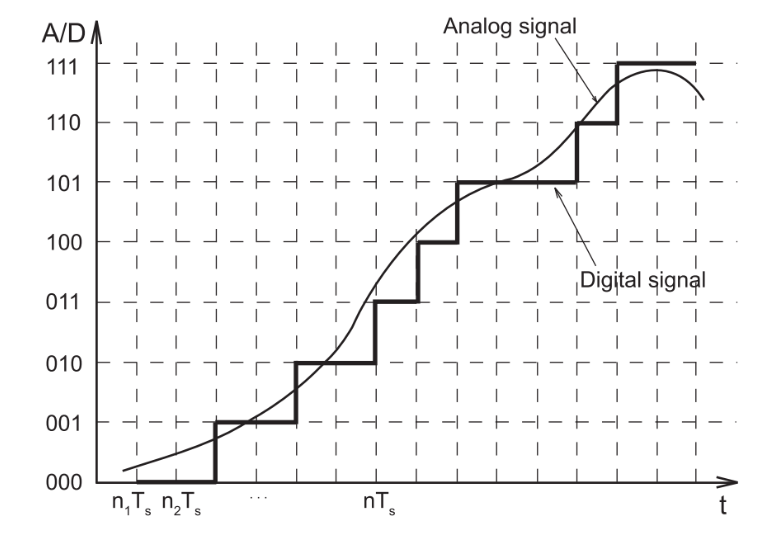
\includegraphics[scale=0.5]{images/ADC.png}
\caption{Analog to Digital Conversion}
\label{fig:x Conversion)}
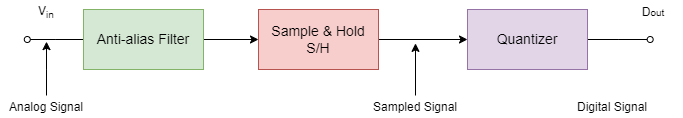
\includegraphics[scale=0.5]{images/ConversionChain.png}
\caption{Analog to Digital Conversion series}
\label{fig:x Conversion series)}
\end{figure}

\section{ADC Characteristics}
ADCs have various characteristics and parameters that define their performance and behavior.  These characteristics are crucial for understanding the capabilities and limitations of an ADC. We have studied several books and articles \cite{ADC_Param},\cite{Acquistion_Eren},and \cite{DAQ_Fundamental} to explore the ADC fundamental, characteristics and parameters. Some of this gist are listed below:
\vspace{1\baselineskip}\par 
\textbf{Resolution:} Resolution is one of the most critical characteristics of an ADC. It refers to the number of bits in the digital output code produced by the ADC. A higher resolution means more bits and greater precision in representing the analog signal. The resolution determines the number of discrete levels or steps into which the ADC can divide the input voltage range. It is the proportion of the change in the input analog voltage to the change in the digital output by one LSB.
\begin{align}
    Resolution = V_{FS} / 2^n -1
\end{align}
Here, $V_{FS}$ is the Full scale input voltage, and n is the number of bit for ADC.
The resolution of a measurement influences its accuracy. The measurement data are more accurate the higher the digitizer resolution. Let's look at what a waveform might be like after being processed by digitizers with various resolutions. Figure \ref{fig:x Resolution Comparison} illustrates the responses of 12, 14, and 16 bits of a typical digitizer to a section of a 200 mV damped sine waveform.

\begin{figure}[htbp]
\centering
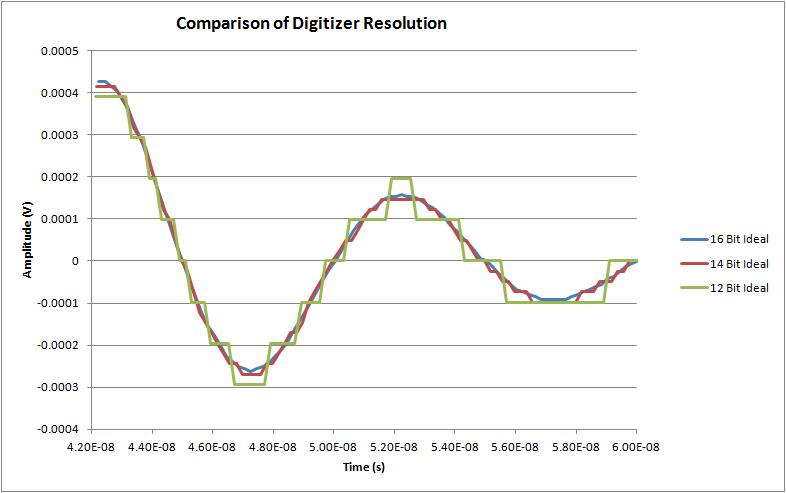
\includegraphics[scale=0.4]{images/Resolution.png}
\caption{A comparison of digitizer resolution on measurement precision}
\label{fig:x Resolution Comparison}
\end{figure}

\vspace{1\baselineskip}\par 
\textbf{Sampling Rate:} The sampling rate is the number of samples taken per unit time by the ADC. It represents how frequently the ADC captures the analog signal. The sampling rate is typically measured in samples per second (SPS) or kilohertz (kHz). A higher sampling rate allows the ADC to capture and represent higher-frequency components of the analog signal accurately. To satisfy the Nyquist-Shannon sampling theorem, the sampling rate must be at least twice the highest frequency component present in the analog signal. This ensures that the digital samples can accurately represent the original analog signal without introducing aliasing or loss of information. For example, if an analog signal contains frequency components up to 10 kHz, the ADC should have a sampling rate of at least 20 kHz to avoid aliasing and accurately capture the signal. The choice of sampling rate depends on the requirements of the application. Higher sampling rates are necessary for accurately capturing high-frequency signals or for applications that require fine time resolution. However, higher sampling rates also result in increased data processing and storage requirements.

\vspace{1\baselineskip}\par 
\textbf{Accuracy:} The ADC's accuracy measures how closely the digital output corresponds to the actual analog input. Numerous elements, including linearity, gain error, offset error, and noise, have an impact on it. There won't be many differences or mistakes between the input and output values of an accurate ADC. The least significant bits (LSBs) or a percentage are commonly used to describe an ADC's accuracy.

\vspace{1\baselineskip}\par 
\textbf{Linearity:} The level of linearity in an ADC refers to how closely the analog input voltage and matching digital output code follow a straight line connection. For similarly spaced analog input voltages, the ADC should generate consistently spaced digital steps. The ideal transfer function may, however, deviate due to flaws in the ADC that cause nonlinearity. Integral nonlinearity (INL) or differential nonlinearity (DNL), which measure the greatest departure from the ideal transfer function, are frequently used to measure the linearity of an ADC.

\vspace{1\baselineskip}\par 
\textbf{Gain Error:} The gap between the ADC's real gain and its ideal gain is known as gain error. Scaling mistakes are introduced into the digital output code. Gain error is frequently quantified in terms of LSBs or percentages.

\vspace{1\baselineskip}\par 
\textbf{Offset Error:} Offset error is the difference between the actual zero-voltage intercept and the transfer function of the ADC. It can be represented as a voltage or LSB value and reflects an added error to the measured value. When there is no input signal, offset error is what causes the offset or shift in the digital output code.

\vspace{1\baselineskip}\par 
\textbf{Signal-to-Noise Ratio:} SNR is a metric that expresses the strength of the intended signal in relation to the noise level at the ADC output. Decibels (dB) are frequently used to express it and are used to measure the amount of noise in the digital output. Better signal integrity and lower noise levels are indicated by a greater SNR.

\vspace{1\baselineskip}\par 
\textbf{Total Harmonic Distortion:} The amount of harmonic distortion the ADC introduces when converting an analog signal to a digital signal is measured by THD. When there are additional frequency components in the output signal that weren't in the analog signal's original version, it's known as harmonic distortion. The amount of distortion in the digital output is indicated by THD, which is given as a percentage or in dB.


\section{ADC architectures}
There are several distinct ADC designs that may be employed for certain application requirements. They are characterized by the rate of sampling or the total amount of clock cycles required to convert a single digital word and resolution. After studying the research paper \cite{KozminPhD}, we have acknowledged that ADC designs are commonly classified into four groups based on sample speed, which has been specified below.
\vspace{1\baselineskip}\par 
\textbf{Slow ADC:} Integrating ADCs have the slow converting speed (2N clock oscillations per data word) but the greatest resolution, which is often greater than 14 bits.\par

\textbf{Medium ADC:} To convert a single sample, a sequential approximations ADC needs N clock cycles. The possible resolution is in the 8-14 bit range.
\par

\textbf{Fast ADC:} This category includes flash, pipeline, subranging, and time-interleaved ADCs. One sample is converted in one to two clock periods. These ADCs generally have resolutions ranging from 6 to 12 bits.\par

\textbf{Oversampling ADC:} Oversampling ADCs, also known as noise- forming ADCs, utilize delta-sigma. Its conversion speed and resolution fall in between those of slow and medium ADCs.\par
\begin{figure}[htbp]
\centering
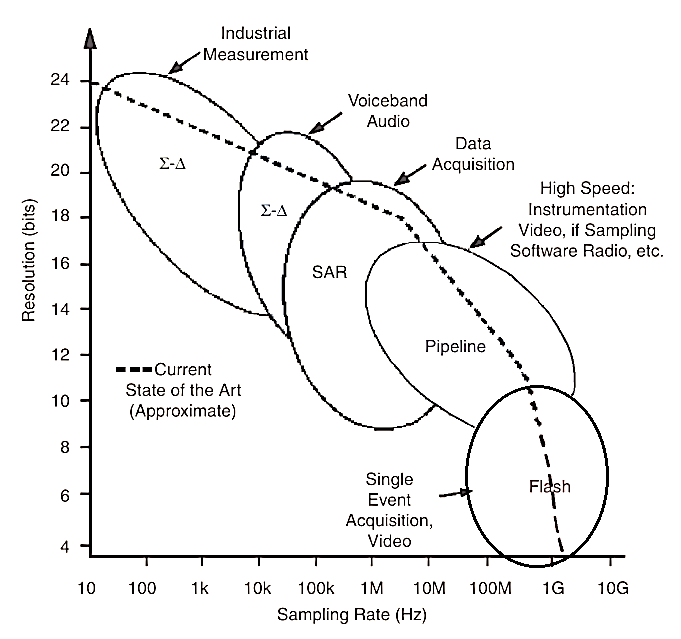
\includegraphics[scale=0.6]{images/ADC Archi.PNG}
\caption{ADC architectures, applications, resolution, and sampling rates.}
\label{fig:x ADC architectures}
\end{figure}

\subsection{Integrating ADC}
There are two techniques to realizing integrating ADCs: single slope and dual slope.These two ADCs interact by integrating a continuous reference signal. Dual Slope ADCs employ integration techniques to calculate the input voltage by measuring the time required for charging or discharging a capacitor. ADCs with dual slopes give high-resolution readings with outstanding noise suppression. They integrate upwardly from an unidentified voltage and then downwards with a knowing voltage source.These are more precise than single sloped ADCs, becuase component defects are wiped away during the de-integration process.Figure \ref{fig:x Dual Slope} is an illustration of slope integration. This charges a capacitor with an electrical current equal to the input voltage over a specific amount of time. The time needed for discharging the identical capacitor at a constant current then establishes the input voltage value. Since it is based on the proportion of ascending time to descent time rather than the true value of the capacitor or other elements whose values fluctuate with temperature and time, the approach is generally precise and reliable.

\begin{figure}[htbp]
\centering
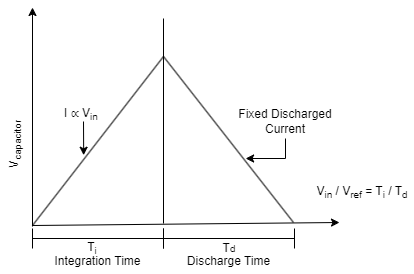
\includegraphics[scale=0.6]{images/Slope.png}
\caption{Dual-Slope ADC Integration and
Discharge Times}
\label{fig:x Dual Slope}
\end{figure}

While an integration timing matches to a multiple of the ac periods, the impact of noise pickups on the ac line's frequency is reduced through integrating the ADC input over an interval. It is frequently utilized in panels meter and precise digital multimeters because to this. Even while conversion rates of up to 60 Hz are typical for 20-bit accuracy, they can be slower for ADCs that integrate across multiples of the line frequencies.

\subsection{Successive-Approximation ADC}
A digital-to-analog converter (DAC), one comparator, controlling logic, and registers make up a successive-approximation converter (Figure \ref{fig:x Successive-Approximation ADC}). The logic initializes the DAC to zero before beginning to count up and set each bit after that until it's reached the current state of the input voltage being monitored \cite{DAQHandbook}. The final value is then recorded in the register when the conversion is complete.The system's logic for control first sets every bit to zero whenever the analog voltage that needs to be assessed is present at the comparator's input.The DAC's output is therefore forced to Half of full scale (as an example of a 10 V full-scale system, the DAC outputs 5.0 V) when the most significant bit (MSB) is set to 1.The comparator subsequently evaluates the analog result of the DAC and compared it to the incoming signal; if the output of the DAC is less than the input signal (which is the signal is more than 1/2 full scale), the MSB is kept at 1.The MSB restores to zero when the output of the DAC is greater than the input signal. Following that, the second MSB, which has a weight of 1/4 of full scale, goes on (sets to 1) and pushes the output signal of the DAC to either 3/4 full scale (if the MSB stayed at 1) or 1/4 full scale (if the MSB restore to zero).Another time, the comparator checks the DAC output to its input signal; if the DAC output is greater than the input, the subsequent bit is reset to zero; otherwise, it remains on (sets to 1). The method then proceeds in order of decreasing bit weight till the LSB is contrasted, after which the 3rd MSB is compared in a similar fashion. The resultant register stores the digital code that represents the analog input signal at the final stage of the procedure.

\begin{figure}[htbp]
\centering
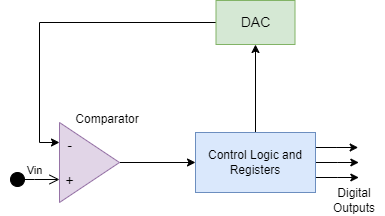
\includegraphics[scale=0.6]{images/SAD.png}
\caption{Successive-Approximation ADC}
\label{fig:x Successive-Approximation ADC}
\end{figure}
Comparisons are performed serially in Successive-Approximation ADC,also they must pause after each step to initialize the DAC and wait for its output to stabilize. Thats why these ADCs are relatively slow.Progressive approximation Because comparisons are performed serially, ADCs are rather sluggish because they must pause after each step to initialize the DAC and wait for its output to stabilize. However, the rate of conversion frequently exceed 1 MHz. Additionally, 12 and 16-bit successive-approximation ADCs are affordable, which explains their widespread use in numerous PC-based collection systems.


\subsection{Flash ADC}
A bunch of parallel connected comparators ($2^N-1$) shown in figure \ref{fig:x Flash ADC}, each with a unique reference level constructs flash ADC.
\begin{figure}[htbp]
\centering
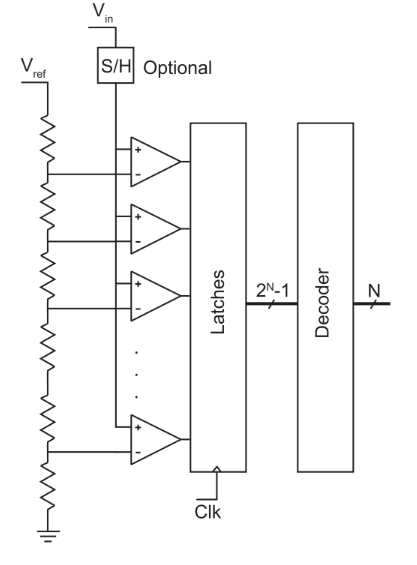
\includegraphics[scale=0.6]{images/Flash.PNG}
\caption{Flash ADC structure}
\label{fig:x Flash ADC}
\end{figure}
The output of the comparator arrays resembles a thermometer because it includes $2^N-1$ bits for every comparator, and each One indicates that the signal is higher than the associated reference value. Afterwards, the decoder converts this code into a binary format. The core component of a Flash ADC is an array of high-speed comparators. Each comparator in the array compares the input analog voltage with a set of reference voltages.The number of comparators in the array directly determines the ADC's resolution.The outputs of the comparators represent the comparison results. For instance, if the input analog voltage is greater than the reference voltage of a comparator, the output is a digital '1'; otherwise, it is a '0'.
\vspace{1\baselineskip}\par 
Flash ADCs are capable of achieving very fast conversion rates, making them suitable for applications requiring high-speed signal processing. They have low conversion latency, which is important in real-time signal processing systems.They can achieve high resolution since each comparator bit contributes to the overall ADC resolution. As the resolution of the ADC increases, the number of comparators and power consumption also increase significantly. Despite its many advantages, Flash ADC has several drawbacks.As the ADC resolution grows, the number of comparators and required precision of the reference voltages become challenging to manage.
\subsection{Delta-sigma ADC}
A high-resolution ADC, known as a Sigma-Delta ADC exploits the oversampling approach to obtain high accuracy in the conversion of analog data to digital format. It consists of a comparator, an integrator, a DAC, and a summing junction, shown in figure \ref{fig:x Delta-sigma ADC} . The fundamental operation of a Sigma-Delta ADC incorporates oversampling the analog input signal at a very high sampling rate, then applying a digital filter to remove noise and retrieve the important data. The digital output data is then generated from the filtered output via decimation.

\begin{figure}[htbp]
\centering
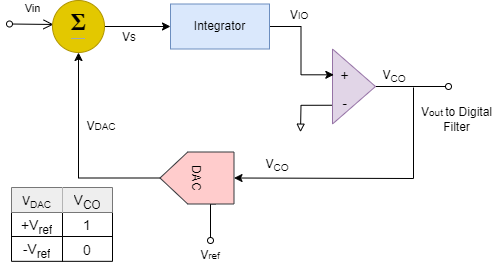
\includegraphics[scale=0.6]{images/Sigma.png}
\caption{Delta-sigma ADC structure}
\label{fig:x Delta-sigma ADC}
\end{figure}





\nomenclature{$LSB$}{Least Significant Bit}
\nomenclature{$SPS$}{Samples Per Second}
\nomenclature{$dB$}{Decibel}
\nomenclature{$SNR$}{Signal-to-Noise Ratio}
\nomenclature{$THD$}{Total Harmonic Distortion}
\nomenclature{$DAC$}{Digital-to-analog converter}
\nomenclature{$MSB$}{Most significant bit}